\documentclass[a4paper, 10pt]{article}

\usepackage{tabularx} % extra features for tabular environment
\usepackage{amsmath}  % improve math presentation
\usepackage{graphicx} % takes care of graphic including machinery
\usepackage[margin=1in,letterpaper]{geometry} % decreases margins
\usepackage{cite} % takes care of citations
\usepackage[final]{hyperref} % adds hyper links inside the generated pdf file
\usepackage{ctex}
\usepackage{titlesec}
%\usepackage{CJKutf8, CJK}
\usepackage{makecell}                 % 三线表-竖线
\usepackage{booktabs}                 % 三线表-短细横线
% \usepackage{natbib}
\usepackage{graphicx}				  % 表格单元格逆时针
\usepackage{multirow}				  % 合并单元格
\usepackage{array}
\usepackage{amssymb}				  % 勾
\usepackage{amsmath}
\usepackage{longtable}                % 导入 longtable 宏包,表格自动换行
\usepackage{caption}
\usepackage{subcaption}               % 设置子图
\usepackage{color}					  % 文本颜色包
\usepackage{xcolor}
\usepackage{bbm}					  % 输入指示函数
\usepackage{tablefootnote}			  % 表格注释
\usepackage{pythonhighlight}
\usepackage{fancyhdr}
\usepackage{lastpage}
\pagestyle{fancy}
\fancyhf{}
\fancyhead{}
\fancyfoot{}
\fancyhead[R]{\small Page \thepage\ of \pageref*{LastPage}}
\fancyhead[L]{\small Report}

\usepackage{listings}                 % 导入代码块
\usepackage{xcolor}
\lstset{
	numbers=left, 
	tabsize=1,
	columns=flexible, 
	numberstyle=  \small, 
	keywordstyle= \color{ blue!70},
	commentstyle= \color{red!50!green!50!blue!50}, 
	frame=shadowbox, % 阴影效果
	rulesepcolor= \color{ red!20!green!20!blue!20} ,
	escapeinside=``, % 英文分号中可写入中文
	xleftmargin=2em,
	xrightmargin=2em, 
	aboveskip=1em,
} 

\hypersetup{
	colorlinks=true,       % false: boxed links; true: colored links
	linkcolor=blue,        % color of internal links
	citecolor=blue,        % color of links to bibliography
	filecolor=magenta,     % color of file links
	urlcolor=blue         
}
%++++++++++++++++++++++++++++++++++++++++
\titleformat{\section}{\Large\bfseries\songti}{\thesection}{1em}{}
\titleformat{\subsection}{\large\bfseries\songti}{\thesubsection}{1em}{}
\titleformat{\subsubsection}{\normalsize\bfseries\songti}{\thesubsubsection}{1em}{}
\titleformat{\paragraph}{\small\bfseries\songti}{\paragraph}{1em}{}
\titleformat{\subparagraph}{\footnotesize\bfseries\songti}{\subparagraph}{1em}{}

\begin{document}
	
	
	\title{\songti \zihao{4}本科生论文设计方向}
	\author{\textrm{Ku Jui}}
	\date{\textrm{October 2023}}
	\maketitle
	
	\renewcommand{\figurename}{Figure} % 可以重新定义abstract,因为ctex会覆盖thebibliography
	% 	\begin{abstract}
		%		In this experiment we studied a very important physical effect by measuring the
		%		dependence of a quantity $V$ of the quantity $X$ for two different sample
		%		temperatures.  Our experimental measurements confirmed the quadratic dependence
		%		$V = kX^2$ predicted by Someone's first law. The value of the mystery parameter
		%		$k = 15.4\pm 0.5$~s was extracted from the fit. This value is
		%		not consistent with the theoretically predicted $k_{theory}=17.34$~s. We attribute %this
		%		discrepancy to low efficiency of our $V$-detector.
		%	\end{abstract}
	\renewcommand{\contentsname}{目录}
	\renewcommand{\tablename}{Table}
	\tableofcontents  % 自动生成目录
	
	\part{Pre-Knowledge}	
	

	\section{背景介绍}
	
	弱光图像增强(Low-light image enhancement, LLIE)是图像处理中的一个重要任务,其目标是提升在低光环境下拍摄的图像的感知质量。这个领域的近期进展主要由深度学习方法主导,包括不同的学习策略、网络架构、损失函数和训练数据。
	
	低光图像增强在不同领域享有广泛的应用,包括视觉监控、自动驾驶和计算摄影。特别是,智能手机摄影已经变得无处不在和突出。受限于相机光圈的大小、实时处理的要求以及存储器的约束,在昏暗环境中用智能手机的相机拍摄照片尤其具有挑战性。
	
	用于低光增强的传统方法包括基于直方图均衡的方法和基于 Retinex 模型的方法。然而,这些方法存在一些局限性,例如在 Retinex 模型中通常忽略噪声,因此在增强结果中保留或放大噪声;找到有效的先验或正则化是具有挑战性的,不准确的先验或正则化可能导致增强结果中的伪像和颜色偏差;由于其复杂的优化过程,运行时间相对较长。
	
	近年来基于深度学习的 LLIE 取得了引人注目的成功。基于深度学习的解决方案比传统方法具有更好的准确性、鲁棒性和速度,因此越来越受到关注。然而,现有的低光照图像增强技术聚焦于构建数据驱动的深度网络,通常其网络模型复杂,导致计算效率低、推理速度慢,并且由于对于训练数据分布的依赖性导致其在未知场景下的性能缺乏保障。
	
	为了解决这些问题并推动该领域的发展,研究者们提出了一些新颖的方法和工具。例如,他们提出了一个大尺度低光图像与视频数据集,并开发了一个包含多种主流 LLIE 方法的在线平台。这些工具可以帮助研究者和开发者更好地理解和改进现有技术,并为未来研究提供宝贵资源。

	\section{前期调研工作}
	
	\paragraph{Attention in CV}
	
	在计算机视觉领域,研究人员使用了不同类型的注意力机制,目的是使模型聚焦于图像本身。这大致分为两种类型:一种是基于通道的注意力机制,即 Squeeze-and-Excite。另一个是基于空间的注意力机制\cite{woo2018cbam}。然而,研究发现这些类型有三个局限性:
	
	\begin{itemize}
		\item[(1)] 
		卷积捕捉远距离特征的能力较差;
		
		\item[(2)]
		注意力机制关注所有输入;当分辨率较大时,计算成本增加;
		
		\item[(3)]
		不同时关注通道和空间维度关注信息。这就造成了信息的浪费和注意力的减弱。
	\end{itemize}	
	
	针对第一个限制 \cite{ramachandran2019stand} 将所有卷积替换为独立的自注意层和空间意识的独立自注意层,替换后的模型为纯注意模型。纯注意模型增强了网络对远距离特征连接的建模能力。在 ImageNet分类任务和 COCO 对象检测任务中,该模型优于使用卷积的基线模型。对于第三个限制,Woo 等人\cite{woo2018cbam}提出了一种卷积块注意模型 CBAM,这是一种轻量级的通用注意模型。该模型从通道维度和空间维度两方面关注重要信息。由于 CBAM 从多个维度提取重要信息,该模型被广泛应用于目标检测、目标分类等任务。实验表明,CBAM 模块可以显著提高网络的表达能力。同时,CBAM 可以搭配 SCConv\cite{li2023scconv}结构,SCConv 是一种名为可以即插即用的卷积模块,目的是减少卷积神经网络中特征之间的空间和通道冗余,从而压缩 CNN 模型并提高其性能。
	
	\paragraph{U-Net for LLIE}
	
	U-Net 网络由卷积层、下采样、上采样和跳过连接操作组成,其编码器和解码器具有对称结构。长期以来,U-Net 网络及其改进结构由于其强大的特征学习和特征重构能力,在图像语义分割领域取得了巨大的成功。U-Net 网络在弱光图像增强方面显示出出色的效果。Chen 等\cite{chen2018learning}创新性地提出了一种基于 U-Net 框架的弱光图像增强网络。该网络的核心架构是多尺度上下文聚合网络 (CAN) 和 U-Net 网络。之后的工作\cite{chen2018learning, zamir2021learning}也将 U-Net 架构应用到自己的网络中,其网络包含两个子网。即图像约简子网和感知损失子网,其中图像约简子网具有与\cite{chen2018learning}相同的 U-Net 架构。虽然\cite{chen2018learning, zamir2021learning}在使用U-Net架构增强图像方面取得了一定的效果,但\cite{meng2020gia}认为\cite{chen2018learning, zamir2021learning}网络忽略了全局信息,导致增强图像中的颜色不自然和物体伪影问题。为了改善以往网络的缺陷,利用 U-Net 架构,\cite{meng2020gia}在U-Net的编码器和解码器之间增加了全局信息感知模块(global information awareness module, GIA), GIA 可以将全局信息整合到整个网络中,改善增强图像中的颜色不一致和伪影。经过对\cite{chen2018learning, meng2020gia, zamir2021learning}的仔细研究,基于 U-Net 网络的弱光图像增强方法取得了很好的效果。然而,该网络仍然存在两个局限性:
	
	\begin{itemize}
		\item[(a)] 
		跳过连接只融合相同尺度的特征,导致编码器和解码器之间存在较大的语义差距;
		
		\item[(2)]
		全局上下文信息的连接相对稀缺。
	\end{itemize}	
	
	这两个限制容易导致增强图像的细节丢失、对比度差和颜色信息不准确。Zhou等\cite{zhou2018unet++,zhou2019unet++}改进了 U-Net 架构生成 U-Net++,在 U-Net++ 中将跳跃连接重新设计为一系列嵌套的密集跳跃连接,实现了多个特征的融合,加强了不同层次的特征信息接触。
	
	\paragraph{CNN for LLIE}
	
	CNN 在许多计算机视觉任务中表现出了令人印象深刻的结果。CNN 利用注意力机制\cite{yang2021locally, zhang2020attention}和上下文信息,从原始图像中生成注意感知并提取多尺度特征\cite{li2018multi,zamir2020learning}。基于 CNN 的低光图像增强方法不断发展。例如,基于 CNN 的自适应弱光图像增强框架\cite{li2020visual}极大地增强了图像对比度、颜色和细节信息。然而,现有的基于 CNN 的方法大多侧重于图像亮度、纹理和颜色的恢复\cite{xu2020learning}。由于局部光照不均匀,颜色信息和细节信息丢失严重,容易出现过增强或增强不足的问题。

	\section{方向}
	
	根据目前的文献研究,在 LLIE 任务中,一种方法是采用边缘检测思想来引导弱光图像增强\footnote{为什么要采用图像的边缘图片来指导弱光图像恢复?
	首先,图像边缘图仅需要很少的数据量,其剔除了不相关的信息,保留了图像重要的结构属性。其次,低光图像通常具有很高的对比度,现有的方法可能无法在极暗或极亮的区域恢复图像边缘细节。同时,当物体边缘不清晰时,像素级损失往往会模糊边缘,破坏图像细节。而加入边缘先验可以降低优化外观重构时的不适定程度。最后,人类视觉系统对边缘高度敏感,保留结构信息对图像重建任务的性能至关重要。定义边缘可以通过学习区分黑暗区域的不同物体来指导增强过程,而不仅仅是识别低光区域。通过保留图像中的结构属性,这使得物体之间的可见性更好。},其策略是将边缘图与\textbf{初步恢复的图像}进行串联,然后通过单一的增强网络来实现最终的图像恢复(见Fig. \ref{fig: EEMEFN})。恢复结果的质量往往会受到最后的增强网络设计和初步恢复图像所包含特征与真实图像特征之间的相似度的影响。
	
	\begin{figure}[htbp]
		% read manual to see what [ht] means and for other possible options
		\centering 
		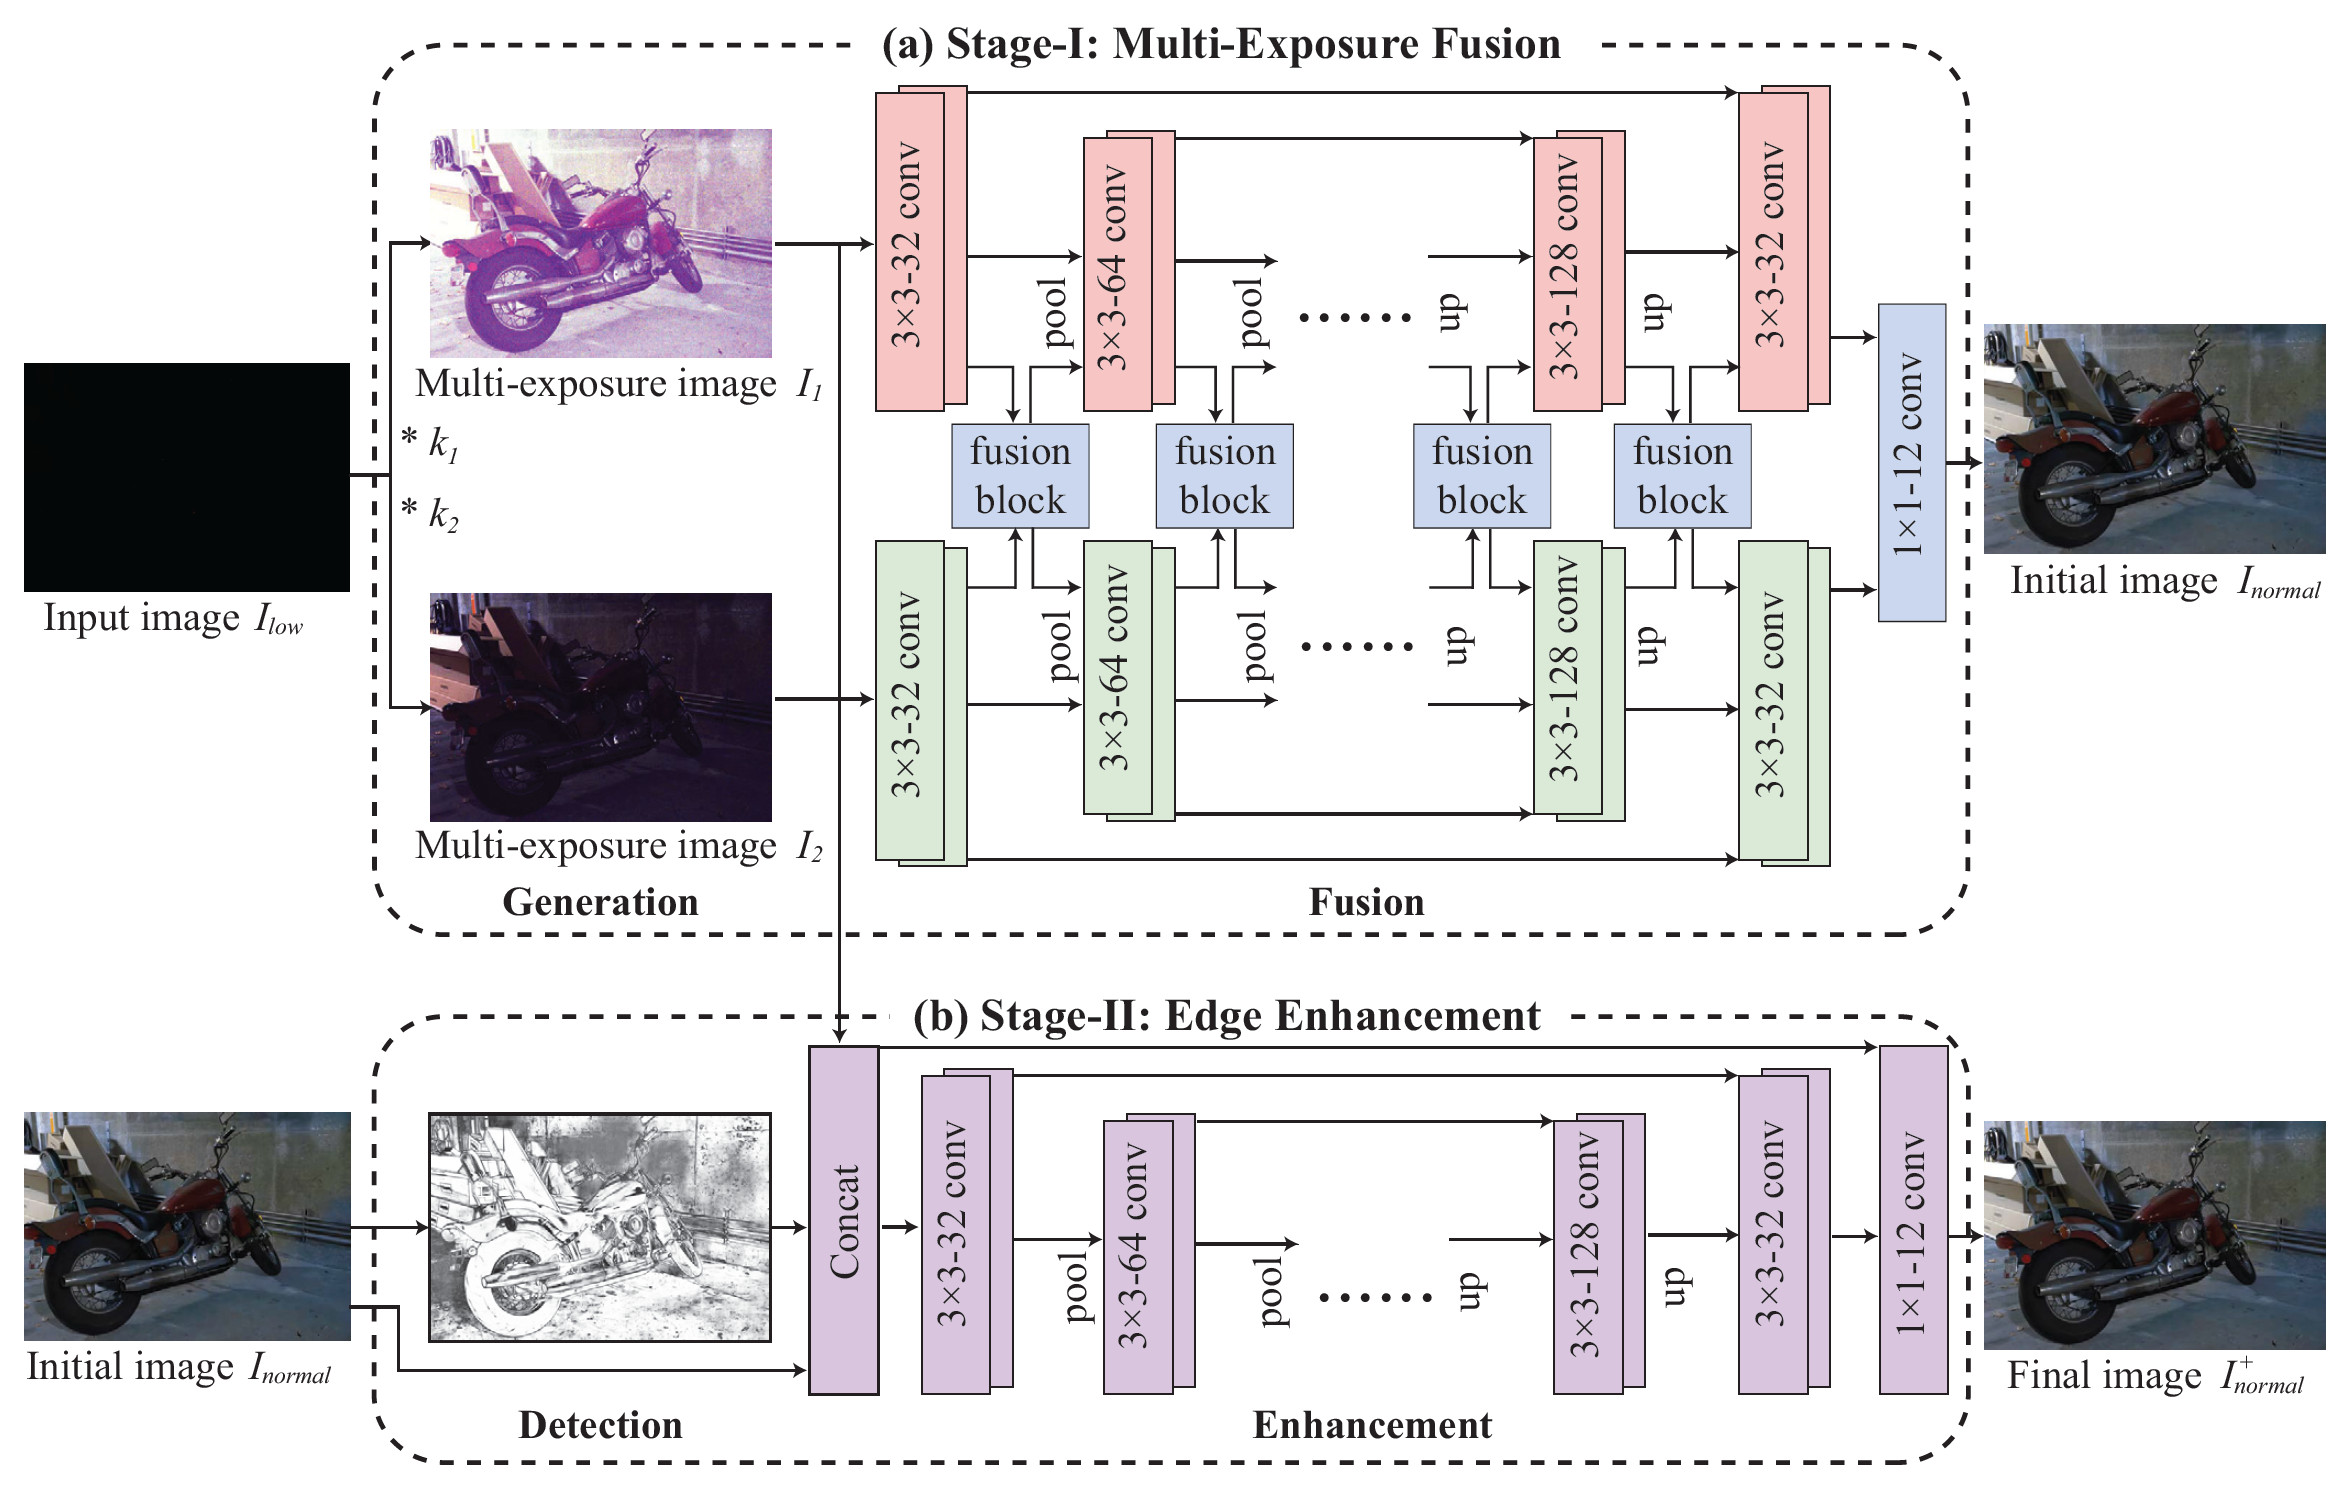
\includegraphics[width=\columnwidth]{picture/LLIE/EEMEFN/EEMEFN framework}
		%\captionsetup{font=scriptsize}
		\caption{
			\label{fig: EEMEFN} 
			该 LLIE 结构源自\cite{zhu2020eemefn},如其 Multi-Exposure Fusion部分采用多曝光融合结构,与由 Initial image 生成的边缘图进行 Concat,后续通过一个 U-Net 网络进一步恢复图像。
		}
	\end{figure}
	
	根据目前的文献调研,当前的此类方法的特点只集中在通过边缘图指导图像恢复,且恢复出来的图像还是有明显噪点。
	
	\subsection{方向一}
	
	\textbf{图像初步恢复的方法}目前主要包括以下几种:
	
	\begin{itemize}
		\item[(1)] 
		利用多曝光技术\footnote{多曝光技术已被实验证明可以有效的解决 LLIE 任务中普遍存在的色彩失真问题。}获得具有不同曝光度的图像,然后结合恢复网络进行初步恢复\footnote{常见的架构如基于 GAN 的多曝光图像融合架构,基于端到端深度学习框架下多曝光图像融合算法,基于稀疏表示和可平移复方向金字塔变换的多曝光融合框架。};
		
		\item[(2)]
		结合 CNN 和 Transformer 架构的方法,可以是类似于 Uformer \cite{wang2022uformer}的串行架构,亦或者是类似于 Conformer 的并行架构。我们提出的 CNN 和 Transformer 并行架构(见Fig. \ref{fig: The proposed architecture})。
		
		\item[(3)]
		直接通过神经网络进行弱恢复。
		
	\end{itemize}	
	
	但由于噪声和伪影的存在,以及色彩与真实图像之间的差异,直接采用神经网络恢复结果通常并不理想。
	
	\begin{figure}[htbp]
		% read manual to see what [ht] means and for other possible options
		\centering 
		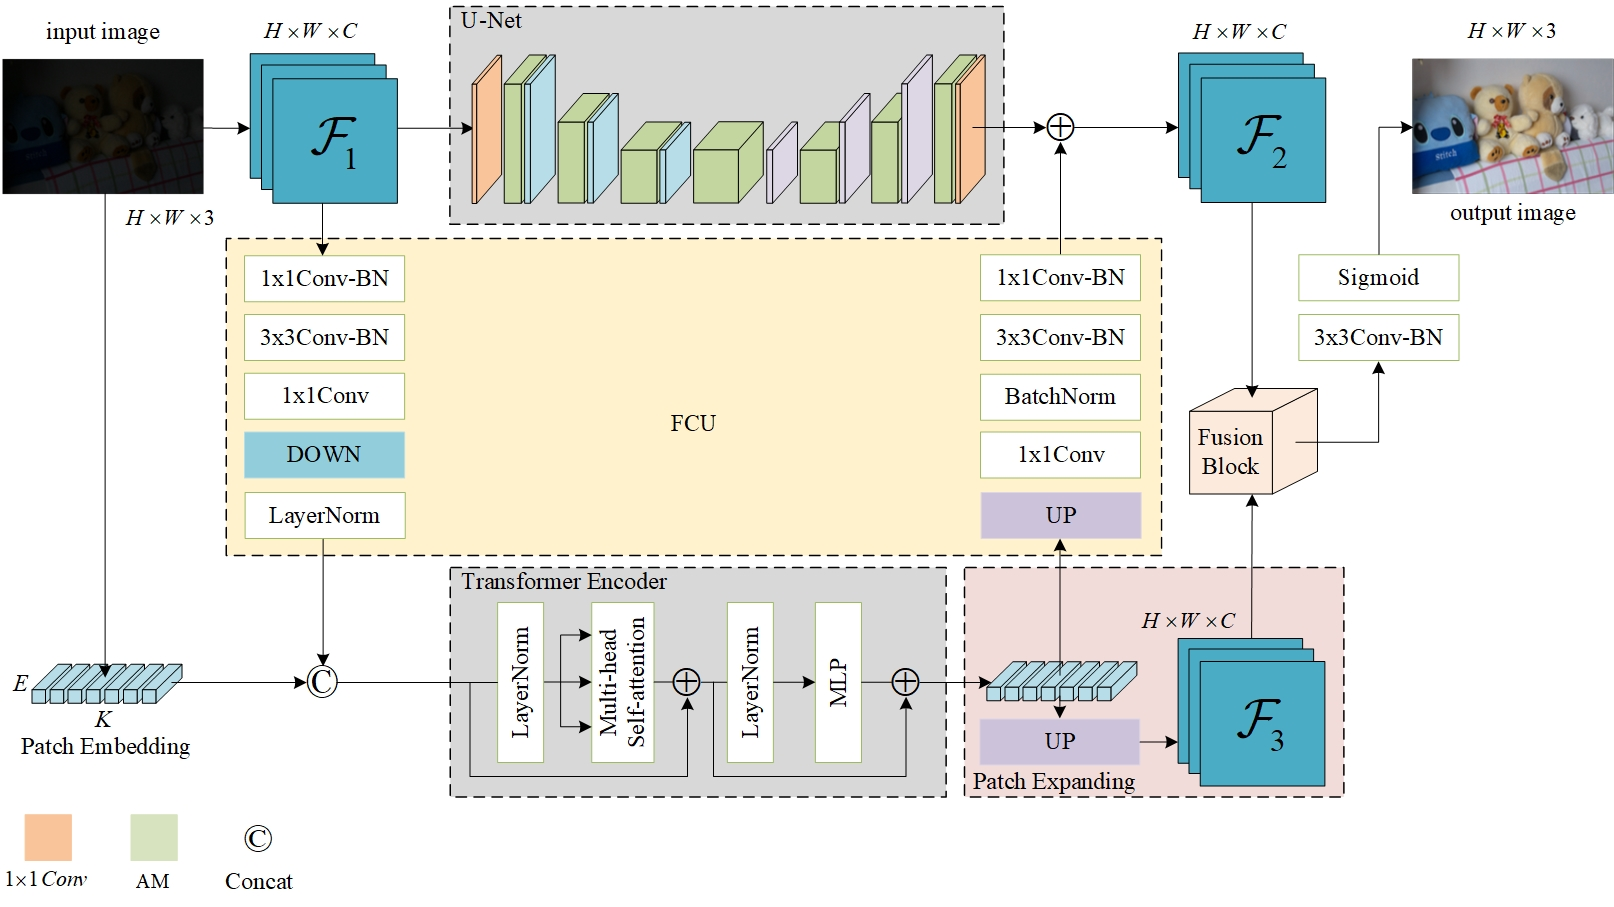
\includegraphics[width=\columnwidth]{picture/LLIE/My Architecture/The proposed initial architecture}
		%\captionsetup{font=scriptsize}
		\caption{
			\label{fig: The proposed architecture} 
			Low-Lighting 图像恢复网络。结构受 Conformer\cite{peng2021conformer} (见 Fig. \ref{fig: Conformer architecture})启发,将原来结构中 CNN 分支的 ResNet 结构修改为 U-Net 结构。其采用一个 U-Net 和 ViT 的并行架构,通过 U-Net 结构得到一个弱恢复的弱特征图 $\mathcal{F}_2$,通过 ViT 融合的特征可以初步增强弱特征图 $\mathcal{F}_2$,ViT 的输出经过 Patch Expanding 的特征图 $\mathcal{F}_3$ 经过与 U-Net 输出的特征图 $\mathcal{F}_2$ 融合之后得到一个初步恢复的图片 output image,用以后续参与图片的进一步恢复。
		}
	\end{figure}
	
	\textcolor{blue}{要求复现 Uformer\cite{wang2022uformer} 代码(见 Fig. \ref{fig: Uformer}),以及基于 Uformer 架构的改进方法\cite{li2023effective}。复现论文\cite{li2023effective}中提出的一种改进的基于 U-Net 网络的弱光图像增强方法(见 Fig. \ref{fig: MCLNet}),作者提出的 CEM 模块本质上基于 Uformer 思想。}。	
	\textcolor{red}{建议拟题《一种基于xx方法的弱光图像增强方法》}
	
	\begin{figure}[htbp]
		% read manual to see what [ht] means and for other possible options
		\centering 
		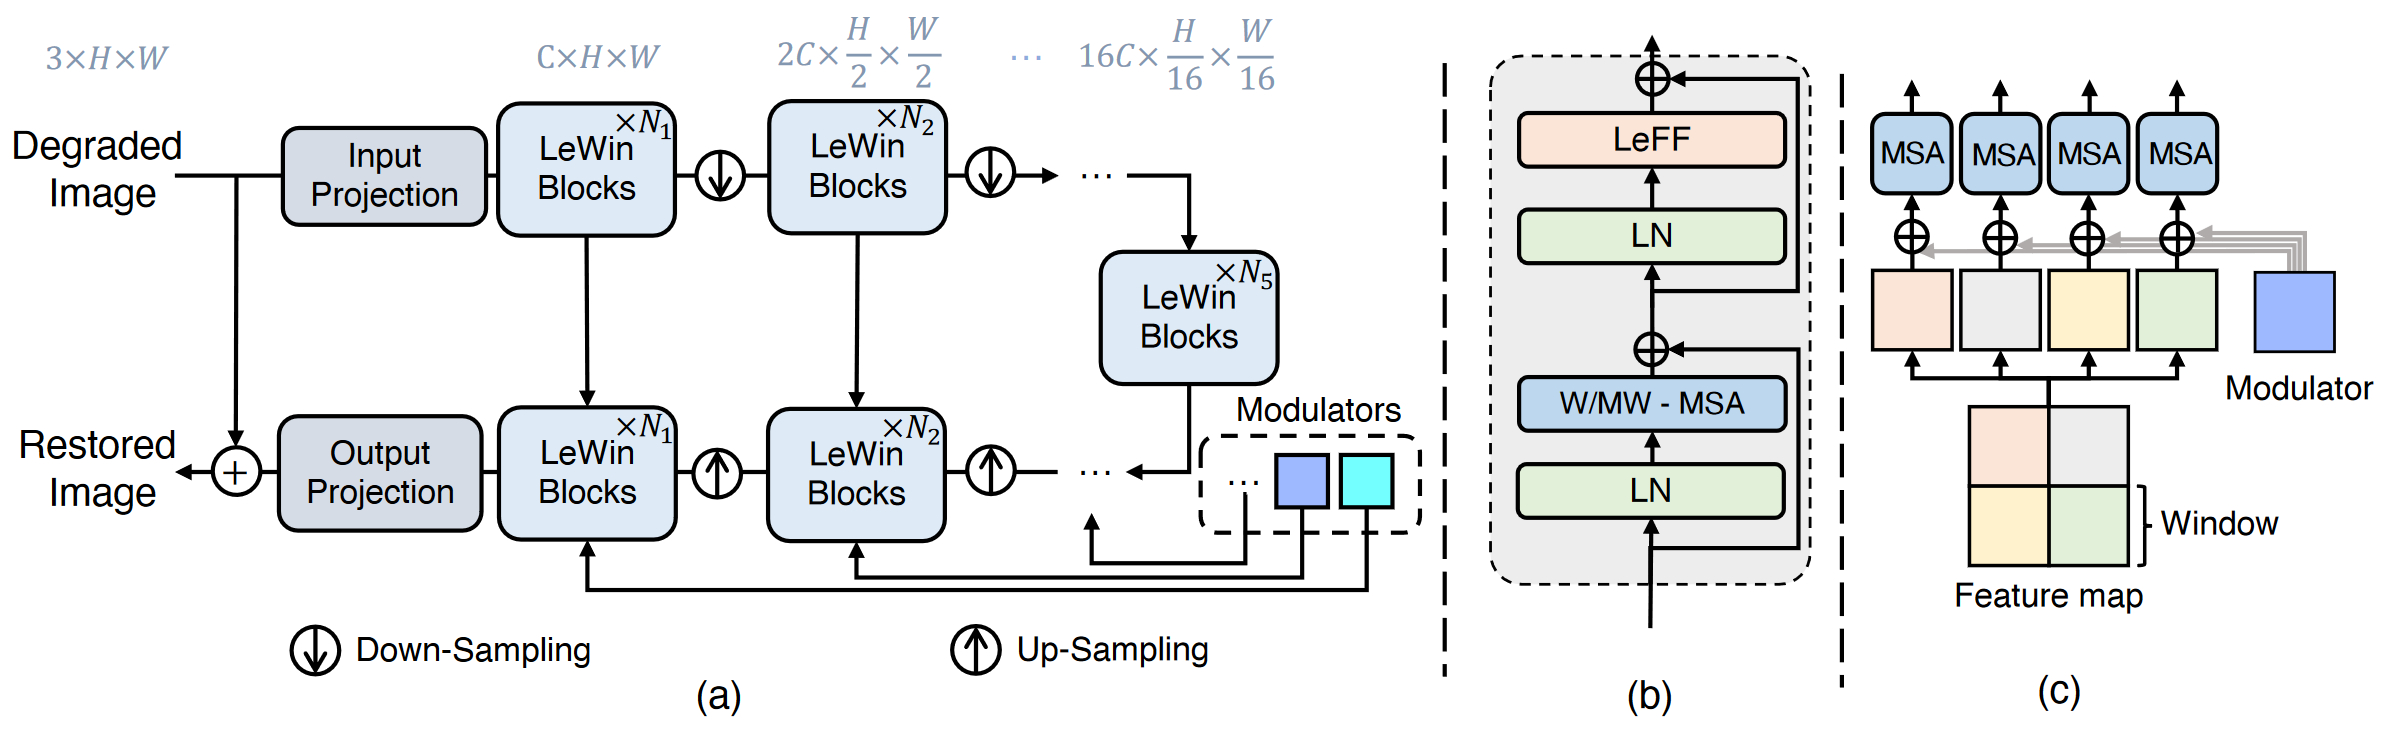
\includegraphics[width=\columnwidth]{picture/LLIE/Uformer/Uformer}
		%\captionsetup{font=scriptsize}
		\caption{
			\label{fig: Uformer} 
			Uformer 的结构。
		}
	\end{figure}
	
	\begin{figure}[htbp]
		% read manual to see what [ht] means and for other possible options
		\centering 
		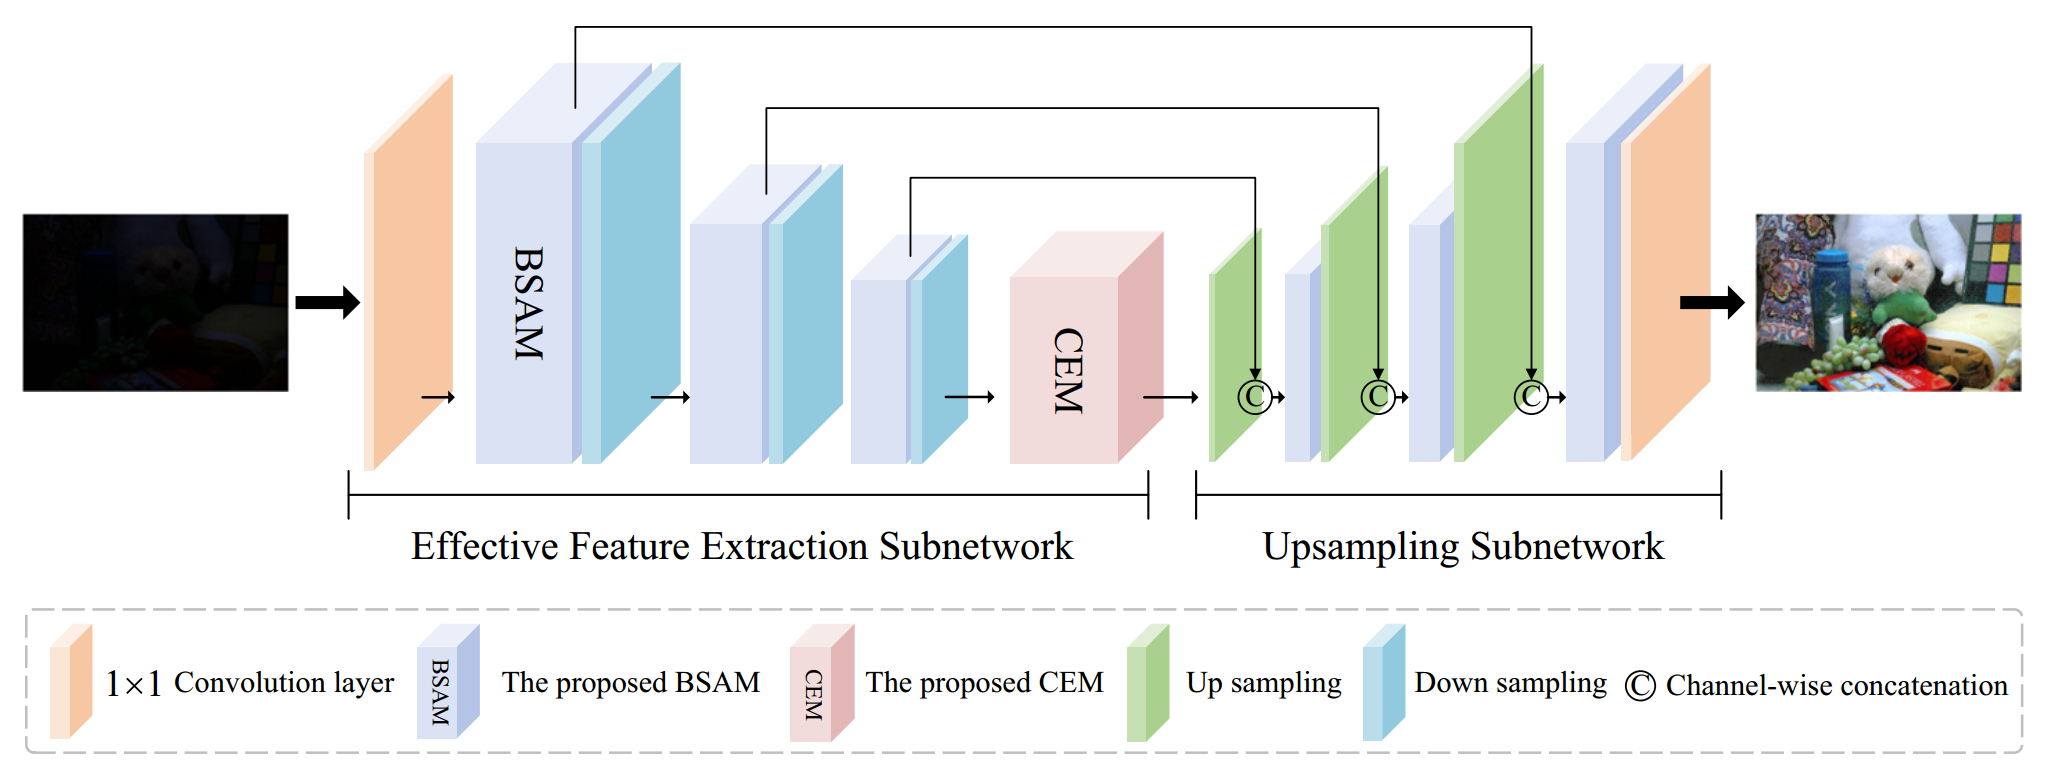
\includegraphics[width=\columnwidth]{picture/LLIE/MCLNet/Overview}
		%\captionsetup{font=scriptsize}
		\caption{
			\label{fig: MCLNet} 
			MCLNet 的结构
		}
	\end{figure}
	
	\subsection{方向二}
	
	此外,\textbf{获取边缘图的方法}也各不相同,在 LLIE 任务中,常见方法采用\textbf{边缘检测网络}来生成边缘图。Canny 和 Sobel 算子通常被用作对比实验,也有一些研究采用辅助边缘网络以提高边缘图生成的准确性。这些方法在弱光图像恢复研究中都具有一定的学术和实际应用价值。目前在 LLIE 领域中获取边缘图分化成了两个不同的方向,一种是采用初步恢复图像获取边缘图(如Fig. \ref{fig: EEMEFN}),另一种是直接采用弱光图像获取边缘图。
	
	\begin{figure}[htbp]
		% read manual to see what [ht] means and for other possible options
		\centering 
		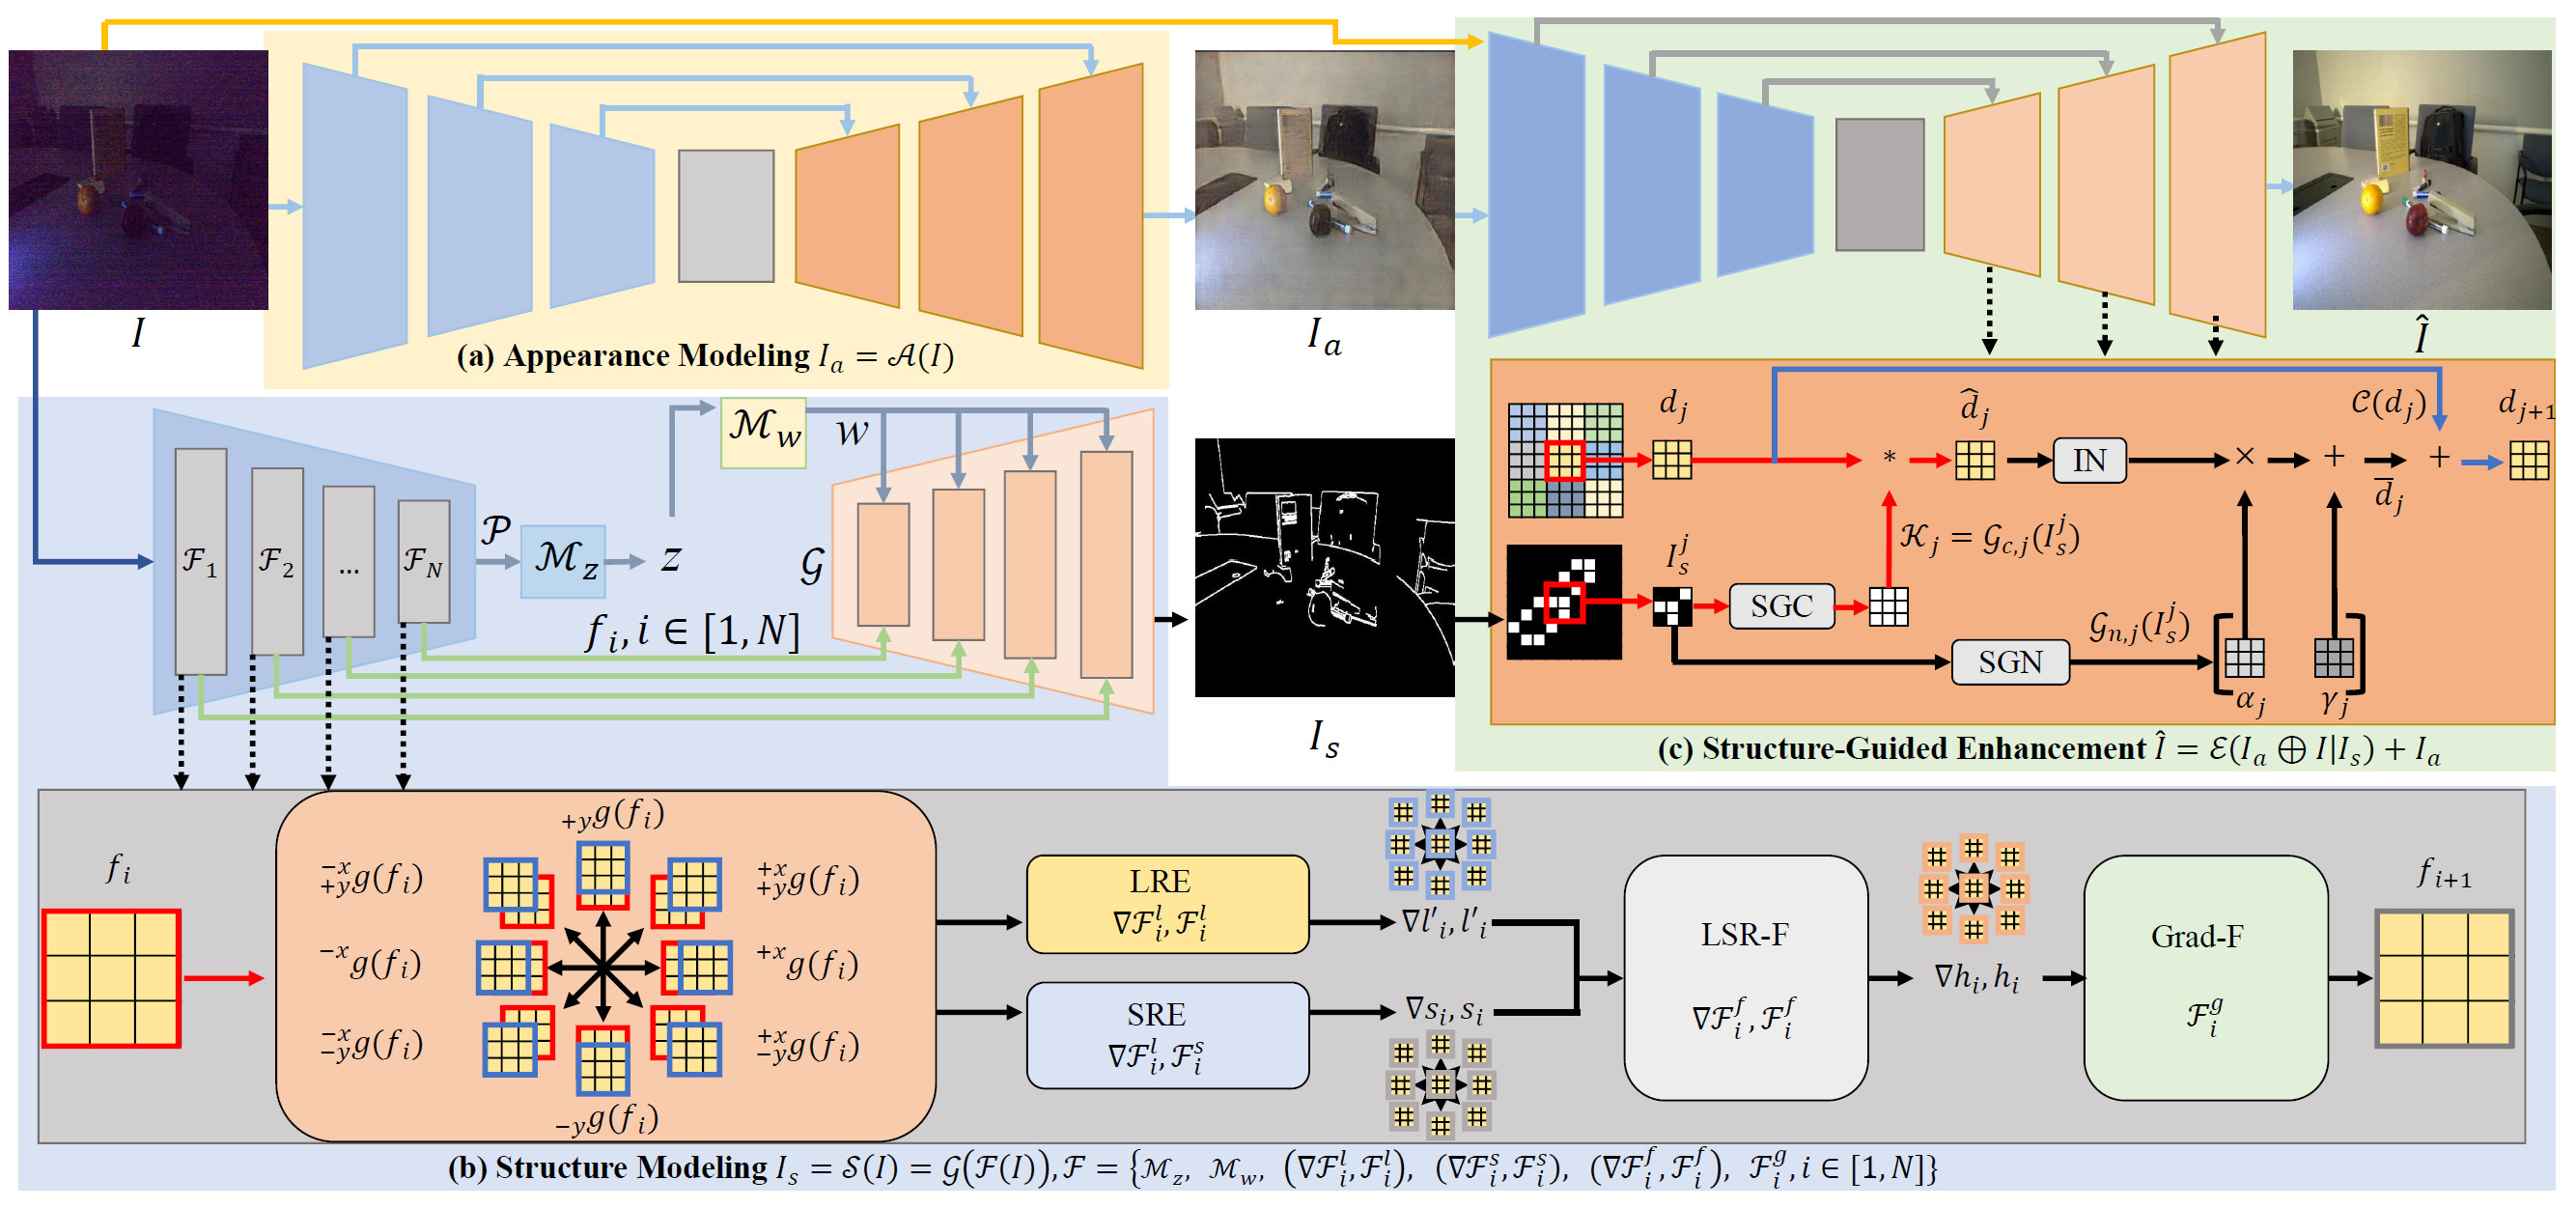
\includegraphics[width=\columnwidth]{picture/LLIE/Structure Modeling and Guidance/Overview}
		%\captionsetup{font=scriptsize}
		\caption{
			\label{fig: Overview} 
			该结构的边缘图直接从 $I$ 中通过 StyleGAN 得到边缘图 $I_s$, 而非从 $I_{\alpha}$ 中通过边缘网络获取边缘图。
		}
	\end{figure}
	
	图像处理任务中边缘检测的各种方法:
	
	\begin{itemize}
		\item[(1)] 
		手工设计各种滤波器来生成边缘图。
		
		\item[(2)]
		根据人类设计的特征使用数据驱动模型来预测边缘(随机决策森林来学习边缘斑块)
		
		\item[(3)]
		深度学习方法从原始数据中学习复杂的特征表示端到端边缘检测模型。
	\end{itemize}	
	
	\textcolor{blue}{要求复现论文\cite{xu2023low}代码。论文作者使用 StyleGAN 结构构建一种边缘网络,可以从弱光图像中获取边缘图。复现论文\cite{zhu2020eemefn}代码,其提出了一个从已经初步恢复的图像(非弱光图像)中获取边缘图的方法。复现论文\cite{rana2021edge},其提出了一种 EdgeNet 方法,可以从弱光图像中获取边缘图的方法。}
	
	\textcolor{red}{建议拟题《一种基于xx方法的弱光图像边缘生成网络》}
	
	\renewcommand{\refname}{References}
	
	
	%	\begin{thebibliography}{00}
		
		%		\bibitem{b1}\label{cite:b1}
		%		W. Wang, C. Wei, W. Yang and J. Liu, "GLADNet: Low-Light Enhancement Network with Global Awareness," 2018 13th IEEE International Conference on Automatic Face \& Gesture Recognition (FG 2018), Xi'an, China, 2018, pp. 751-755, DOI: 10.1109/FG.2018.00118.
		
		%		\bibitem{b2}\label{cite:b2}
		%		A.\ Mahajan, K.\ Somaraj and M. Sameer, "Adopting Artificial Intelligence Powered ConvNet To Detect Epileptic Seizures," 2020 IEEE-EMBS Conference on Biomedical Engineering and Sciences (IECBES), Langkawi Island, Malaysia, 2021, pp. 427-432, DOI: 10.1109/IECBES48179.2021.9398832.
		
		%		\bibitem{Cyr}
		%		N.\ Cyr, M.\ T$\hat{e}$tu, and M.\ Breton,
		% "All-optical microwave frequency standard: a proposal,"
		%		IEEE Trans.\ Instrum.\ Meas.\ \textbf{42}, 640 (1993).
		
		
		
		%	\end{thebibliography}
	
	\bibliographystyle{unsrt}
	\bibliography{reference}
	
	
\end{document}
